\documentclass[10pt,notitlepage]{article}
\usepackage{graphicx}
\usepackage{verbatim}
\usepackage[portuguese]{babel}
\usepackage[utf8]{inputenc}
\usepackage[hmargin=2cm,vmargin=3.5cm,bmargin=2cm]{geometry}
\usepackage{multicol}
\usepackage{hyperref}



\begin{document}

%%%CAPA%%%
\begin{titlepage}
\begin{figure}
\centering

\includegraphics[scale=0.5]{logo.pdf}
\end{figure}



\begin{center}

Escola de Engenharia \\~  Departamento de Informática \\~ \\~ Licenciatura em Engenharia Informática \\~ \\~ \\~  \\~ \\~ \\~ \\~ \\~ \\~ \\~


{\Huge Projecto Java - FitnessUM }
\\~ \\~ \\~ \\
Programação Orientada aos Objectos
  \vfill

\begin{figure}[h]
\centering

\end{figure}

\begin{figure}[h]
\centering
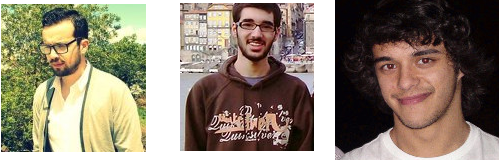
\includegraphics[scale=0.6]{autores.png}
\end{figure}

69303 ~~~~~~~~~~~~~~~~~~ 66822 ~~~~~~~~~~~~~~~~~~~~~ 69854   \\~ Bruno Pereira  ~~~~~~~~ Miguel Guimarães ~~~~~~~João Mano  \\~ \\~ \\~ \\~ \\~ \\~ Braga, Junho de 2014
\end{center}
\end{titlepage}




\tableofcontents

\newpage


\section{Estrutura da aplicação}

\subsection{Actividades}
Foram definidas as seguindes actividades desportivas para a nossa aplicação:
\begin{multicols}{2}
\begin{itemize}
\item Yoga
\item Aerobics
\item Swimming
\item IndoorCycling
\item Handball
\item Basketball
\item TableTennis
\item Boxing
\item Badminton
\item VolleyBallIndoor
\item Football
\item VolleyBallBeach
\item Running
\item Skating
\item Saling
\item Walking
\item Tennis
\item Skiing
\item Cycling
\item MountainBiking
\item Orienteering
\item Snowboarding
\item Polo
\end{itemize}
\end{multicols}

Para a implementação destas actividades foi usada a seguinte estrutura:



\begin{figure}[ht]
\centering
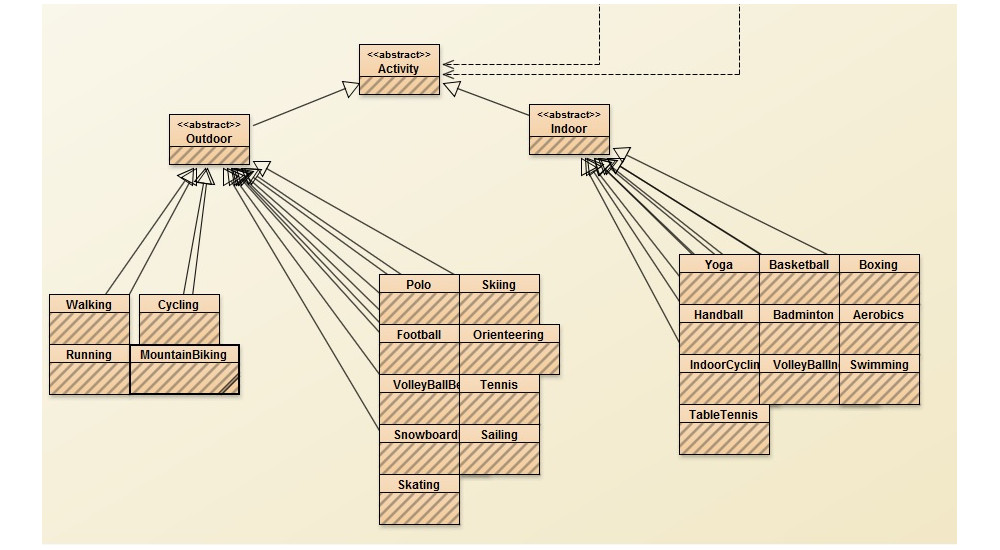
\includegraphics[scale=0.5]{Activity2.jpg}
\caption{Estrutura das actividades}
\label{fig:actividades}
\end{figure}


\subsubsection{Classe abstracta Activity}

Esta é a classe mais abstracta que contem o conceito de actividade. Contém variáveis comuns a todas as actividades:
\begin{itemize}
\item \textit{String name}, nome da actividade criada.
\item \textit{GregorianCalendar date}, data de quando se realizou a actividade.
\item \textit{double timeSpent}, tempo gasto na actividade.
\item \textit{double calories}, campo preenchido pela aplicaçao de uma fórmula.
\end{itemize}
tal como os construtores, \textit{getters} e \textit{setters}.


\subsubsection{Indoor,Outdoor e actividades desportivas}
Todas as actividades desportivas tem um aspecto importante,o clima caso sejam praticadas ao ar livre.\\
Devido a este aspecto foram criadas duas classes abstractas,subclasses de \textit{Activity},para essa distinção.
\begin{itemize}
\item Outdoor,contém a variável: \textit{String weather}
\item Indoor
\end{itemize}

Todas as actividades desportivas são subclasses de \textit{Indoor} ou \textit{Outdoor} como exemplicado na figura ~\ref{fig:actividades}.

\subsubsection{Comparadores e Interfaces}
Para organizar as actividades criaram-se dois tipo de comparadores:
\begin{itemize}
\item CompareActivity- Compara a actividade pela data da realização da mesma.
\item CompareActivityByTime- Compara a actividade pelo tempo gasto na realização desta.
\end{itemize}

\begin{figure}[ht]
\centering
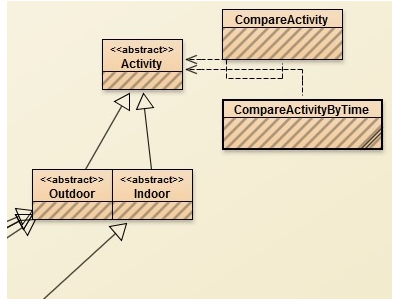
\includegraphics[scale=1]{ComparadorActivity.png}
\caption{Comparador Activity}
\end{figure}

~\\~\\

Depois de uma análise às actividades desportivas, ficou claro que para certas actividades se deviam registar distancias e para outras registar pontuações,neste seguimento foram criadas as seguintes interfaces:



\begin{itemize}
\item UserVs-Interface de métodos relacionados com pontos(pontos próprios e pontos do adversário)
\item Distance -Interface de métodos relacionados com actividades de distancia.
\item VerticalDistance- Interface de métodos relacionados com actividades de distancia vertical

\end{itemize}
\begin{figure}[h]
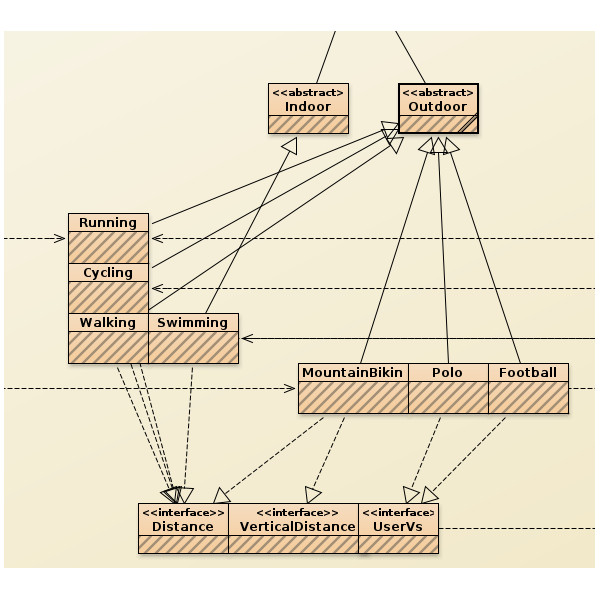
\includegraphics[scale=0.5]{interfaceAct.jpg}
\caption{Exemplo de algumas actividades que implementam as interfaces}
\end{figure}


\subsection{Utilizadores}
Para distinguir utilizadores regulares de administradores criou-se a seguinte estrutura:
~\\
\begin{figure}[htb]
\centering
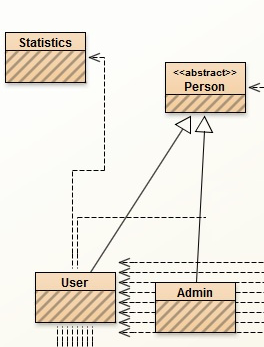
\includegraphics[scale=0.6]{Statsfinal.jpg}
\caption{Estrutura das classes User e Admin}
\end{figure}


\subsubsection{Classe abstracta Person}

~\\~
Classe geral para todo tipo de utilizador. As suas variáveis são:
\begin{itemize}
\item \textit{String email};
\item \textit{String password};
\item \textit{String name};
\item \textit{char gender};
\item \textit{GregorianCalendar dateOfBirth};
\end{itemize}

\subsubsection{Classes User e Admin}

As subclasses de Person referem-se a dois possíveis tipos de utilizador, utilizador normal ou utilizador com privilégios de administrador.\\
A classe Admin não tem métodos ou variáveis adicionais, visto que este tipo de utilizador apenas opera sobre a base de dados da aplicação.\\
A classe User adiciona as seguintes variáveis:
\begin{itemize}
\item \textit{int height};
\item \textit{double weight};
\item \textit{String favoriteActivity};
\item \textit{TreeSet$<$Activity$>$ userActivities} - Actividades realizadas pelo utilizador;
\item \textit{TreeSet$<$String$>$ friendsList} - Lista dos amigos do utilizador;
\item \textit{TreeMap$<$String, ListRecords$>$ records} - Lista dos seus recordes pessoais;
\item \textit{TreeSet$<$String messageFriend} - Lista de pedidos de amizade;
\end{itemize}
Respectivos métodos \textit{getters} e \textit{setters}, construtores e métodos auxiliares para a gestão de amigos/pedidos de amizade, recordes pessoais, das suas actividades e estatísticas relevantes. Ainda contém funções auxiliares para a simulação de eventos.

\subsubsection{Comparators}
O tipo Person tem apenas um comparator:
\begin{itemize}
\item ComparePersonByName - que ordena por ordem alfabética do seu nome.
\end{itemize}
\subsubsection{Statistics}

A classe Statistics é usada para mostrar ao utilizador dados relevantes das suas actividades, estes podem ser descriminados por um dado mês ou por um ano. As suas variáveis são:
\begin{itemize}
\item \textit{double timeSpend};
\item \textit{double calories};
\item \textit{double distance};
\end{itemize}
contém os respectivos métodos \textit{getters} e \textit{setters} e construtores.


\subsection{Recordes Pessoais}
Para registar os recordes chegou-se a estrutura da fig ~\ref{fig:recordes}:
~\\
\begin{figure}[h]
\centering
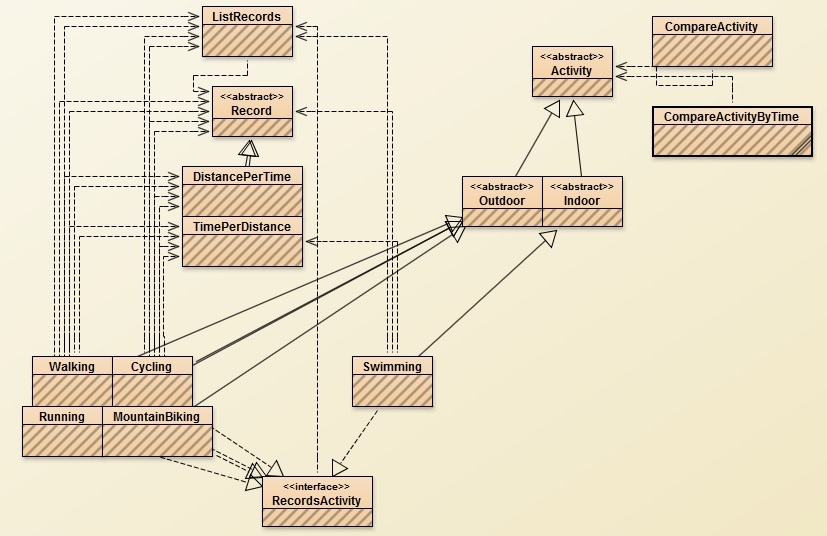
\includegraphics[scale=0.6]{Records.jpg}
\caption{Estrutura dos recordes}
\label{fig:recordes}
\end{figure}


Como se pode verificar na figura ~\ref{fig:recordes}, apenas as seguintes actividades contêm recordes:
\begin{itemize}
\item Running
\item Cycling
\item Walking
\item MountainBiking
\item Swimming
\end{itemize}


\subsubsection{Classe abstracta Record}

Esta classe representa todos os recordes que o utilizador pode bater. Contém apenas uma variável:
\begin{itemize}
\item \textit{String name}-Nome do tipo de recorde a bater(ex: 1km,10 miles,Cooper...)
\end{itemize}
métodos construtores, \textit{getName()} e \textit{isEmpty()} que verifica se esse recorde existe ou não.


\subsubsection{DistancePerTime e TimePerDistance}
Estas classes simbolizam os dois diferentes tipos de recordes.\\

DistancePerTime é um recorde em que o objectivo é fazer a maior distância para um dado tempo.
As suas variáveis são:
\begin{itemize}
\item \textit{double recordTime} - Tempo do recorde;
\item \textit{double distance} - Distância registada;
\end{itemize}
Enquanto que TimePerDistance representa um recorde de menor tempo para uma certa distância.
As suas variaveis sao:
\begin{itemize}
\item \textit{double recordDistance} - Distância do recorde;
\item \textit{double time} - Tempo registado;
\end{itemize}
~\\
Estas duas classes têm os mesmos métodos, no entanto os métodos \textit{update} e \textit{setStatistics}, estão implementados de maneiras diferentes, tendo em conta que em DistancePerTime, quanto maior a distância melhor é o recorde, e no caso do TimePerDistance,  o melhor recorde é o de menor tempo.


\subsubsection{ListRecords}

Classe que agrupa todos os recordes de uma actividade. Tem como variáveis:
\begin{itemize}
\item \textit{String name} - Aqui o nome simboliza o tipo de actividade (Ex: Running, Walking...);
\item \textit{ArrayList$<$Record$>$ recs} - Lista dos recordes;
\end{itemize}
Tem implementado métodos construtores, \textit{getters}, \textit{setters} e ainda um método \textit{updateList()} que aplica a função \textit{update()} a todos os objectos \textit{Record} da lista. (Subsitui na lista original caso recorde da segunda lista seja melhor).
\subsubsection{Interfaces}
Nesta fase,visto que nem todas as actividades desportivas implementarem recordes, chegou-se então à conclusão que estas actividades precisam sempre de devolver a lista de recordes registados,então implementou-se a seguinte interface:
\begin{itemize}
\item \textit{RecordsActivity};
\end{itemize}
Que contém o seguinte método:
\begin{itemize}
\item \textit{getListRecords};
\end{itemize}

\subsection{Fórmulas}
Em certos momentos do trabalho surgiu a necessidade de codificar fórmulas.\\
Tal aconteceu para calcular as calorias gastas em cada actividade e para a simulação dos eventos.

\subsubsection{Fórmula das Calorias}



Sabendo que:\\ \textbf{MET(Metabolic Equivalent of Task)}- Medida fisiológica que expressa o custo energético de cada actividade física.


E usando o seguinte quadro: \url{http://www.cdof.com.br/MET_compendium.pdf}\\
Criou-se a seguinte fórmula:\\

\begin{tabular}{|r|}
  \hline
 \textbf{Calorias}$=mets * pesoDoUtilizador * (tempoGasto(min) / 60)$\\
 \hline \hline
\end{tabular}


\subsubsection{Fórmula para a Simulação}
\end{document}

















